% EfficientNet-B0 / ImageNet-1k validation curve (bf16, 6x 4060 Ti). pgfplots.
\begin{center}
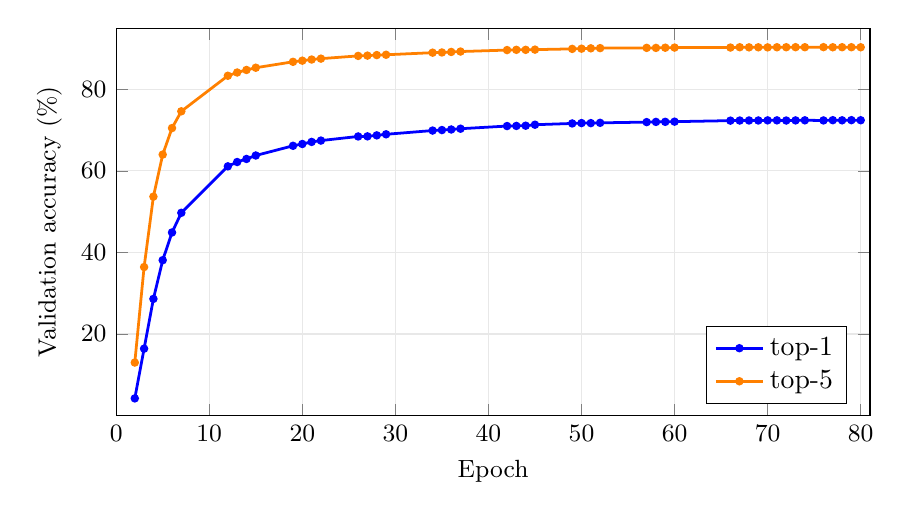
\begin{tikzpicture}
\begin{axis}[
    width=0.92\linewidth, height=6.5cm,
    xlabel={Epoch}, ylabel={Validation accuracy (\%)},
    xmin=0, xmax=81, ymin=0, ymax=95,
    xtick={0,10,20,30,40,50,60,70,80}, ytick={20,40,60,80},
    legend pos=south east, legend cell align={left},
    grid=major, grid style={gray!18},
    tick label style={font=\small}, label style={font=\small},
    every axis plot/.append style={line width=1pt, mark size=1pt},
]
\addplot[blue, mark=*, mark options={fill=blue}] coordinates {
(2,4.20) (3,16.40) (4,28.61) (5,38.10) (6,44.90) (7,49.72) (12,61.12) (13,62.18) (14,62.93) (15,63.78) (19,66.16) (20,66.60) (21,67.11) (22,67.44) (26,68.45) (27,68.48) (28,68.72) (29,68.98) (34,69.90) (35,70.02) (36,70.16) (37,70.35) (42,71.00) (43,71.03) (44,71.09) (45,71.33) (49,71.64) (50,71.73) (51,71.72) (52,71.79) (57,71.97) (58,72.02) (59,72.04) (60,72.08) (66,72.33) (67,72.36) (68,72.37) (69,72.37) (70,72.40) (71,72.40) (72,72.36) (73,72.39) (74,72.41) (76,72.38) (77,72.44) (78,72.41) (79,72.45) (80,72.43)
};
\addlegendentry{top-1}
\addplot[orange, mark=*, mark options={fill=orange}] coordinates {
(2,12.99) (3,36.42) (4,53.69) (5,64.01) (6,70.51) (7,74.62) (12,83.34) (13,84.14) (14,84.76) (15,85.31) (19,86.76) (20,87.04) (21,87.32) (22,87.54) (26,88.21) (27,88.28) (28,88.41) (29,88.49) (34,89.00) (35,89.05) (36,89.18) (37,89.28) (42,89.64) (43,89.70) (44,89.70) (45,89.75) (49,89.93) (50,89.98) (51,90.07) (52,90.12) (57,90.18) (58,90.17) (59,90.22) (60,90.25) (66,90.26) (67,90.34) (68,90.31) (69,90.32) (70,90.30) (71,90.33) (72,90.34) (73,90.35) (74,90.34) (76,90.36) (77,90.33) (78,90.34) (79,90.34) (80,90.33)
};
\addlegendentry{top-5}
\end{axis}
\end{tikzpicture}
\end{center}

\noindent EfficientNet-B0 / ImageNet-1k validation accuracy per epoch (bf16,
6$\times$ 4060 Ti). Final: $\mathbf{72.3\%}$ top-1 / $\mathbf{90.3\%}$ top-5.
